%%%%%%%%%%%%%%%%%%%%%%%%%%%%%%%%%%%%%%%%%%%%%%%%%%%%%%%%%%%%%%%%%%%%%%%%%%%%%%%%%
% Template: Article
%
% Por: Abrantes Araújo Silva Filho
%      abrantesasf@gmail.com
%
% Citação: Se você gostou deste template, por favor ajude a divulgá-lo mantendo
%          o link para meu repositório GitHub em:
%          https://github.com/abrantesasf/LaTeX
%%%%%%%%%%%%%%%%%%%%%%%%%%%%%%%%%%%%%%%%%%%%%%%%%%%%%%%%%%%%%%%%%%%%%%%%%%%%%%%%%




%%%%%%%%%%%%%%%%%%%%%%%%%%%%%%%%%%%%%%%%%%%%%%%%%%%%%%%%%%%%%%%%%%%%%%%%%%%%%%%%%
%%% Configura o tipo de documento, papel, tamanho da fonte e informações básicas
%%% para as proriedades do PDF/DVIPS e outras propriedades do documento
\RequirePackage{ifpdf}
\ifpdf
  % Classe, língua e tamanho da fonte padrão. Outras opções a considerar:
  %   draft
  %   onecolumn (padrão) ou twocolumn (OU usar o package multicol)
  %   fleqn com ou sem leqno (alinhamento à esquerda das fórmulas e dos números)
  %   oneside (padrão para article ou report) ou twoside (padrão para book)
  \documentclass[pdftex, brazil, 12pt, twoside]{article}
\else
  % Classe, língua e tamanho da fonte padrão. Outras opções a considerar:
  %   draft
  %   onecolumn (padrão) ou twocolumn (OU usar o package multicol)
  %   fleqn com ou sem leqno (alinhamento à esquerda das fórmulas e dos números)
  %   oneside (padrão para article ou report) ou twoside (padrão para book)
  \documentclass[brazil, 12pt]{article}
\fi


%%%%%%%%%%%%%%%%%%%%%%%%%%%%%%%%%%%%%%%%%%%%%%%%%%%%%%%%%%%%%%%%%%%%%%%%%%%%%%%%%
%%% Carrega pacotes iniciais necessários para estrutura de controle e para a
%%% criação e o parse de novos comandos
\usepackage{ifthen}
\usepackage{xparse}


%%%%%%%%%%%%%%%%%%%%%%%%%%%%%%%%%%%%%%%%%%%%%%%%%%%%%%%%%%%%%%%%%%%%%%%%%%%%%%%%%
%%% Configuração do tamanho da página, margens, espaçamento entrelinhas e, se
%%% necessário, ativa a indentação dos primeiros parágrafos.
\ifpdf
  \usepackage[pdftex]{geometry}
\else
  \usepackage[dvips]{geometry}
\fi
\geometry{a4paper, left=2.6cm, right=4.0cm, top=3.0cm, bottom=3.4cm}

\usepackage{setspace}
  \singlespacing
  %\onehalfspacing
  %\doublespacing


%%%%%%%%%%%%%%%%%%%%%%%%%%%%%%%%%%%%%%%%%%%%%%%%%%%%%%%%%%%%%%%%%%%%%%%%%%%%%%%%%
%%% Configurações de cabeçalho e rodapé:
\usepackage{fancyhdr}
\setlength{\headheight}{1cm}
\setlength{\footskip}{1.5cm}
\renewcommand{\headrulewidth}{0.3pt}
\renewcommand{\footrulewidth}{0.0pt}
\pagestyle{fancy}
\renewcommand{\sectionmark}[1]{%
  \markboth{\uppercase{#1}}{}}
\renewcommand{\subsectionmark}[1]{%
  \markright{\uppercase{\thesubsection \hspace{0.1cm} #1}}{}}
\fancyhead{}
\fancyfoot{}
\newcommand{\diminuifonte}{%
    \fontsize{9pt}{9}\selectfont
}
\newcommand{\aumentafonte}{%
    \fontsize{12}{12}\selectfont
}
% Configura cabeçalho e rodapé para documentos TWOSIDE
\fancyhead[EL]{\textbf{\thepage}}
\fancyhead[EC]{}
\fancyhead[ER]{\diminuifonte \textbf{\leftmark}}
\fancyhead[OR]{\textbf{\thepage}}
\fancyhead[OC]{}
\fancyhead[OL]{\diminuifonte \textbf{\rightmark}}
\fancyfoot[EL,EC,ER,OR,OC,OL]{}
% Configura cabeçalho e rodapé para documentos ONESIDE
%\lhead{ \fancyplain{}{sup esquerdo} }
%\chead{ \fancyplain{}{sup centro} }
%\rhead{ \fancyplain{}{\thesection} }
%\lfoot{ \fancyplain{}{inf esquerdo} }
%\cfoot{ \fancyplain{}{inf centro} }
%\rfoot{ \fancyplain{}{\thepage} }




%%%%%%%%%%%%%%%%%%%%%%%%%%%%%%%%%%%%%%%%%%%%%%%%%%%%%%%%%%%%%%%%%%%%%%%%%%%%%%%%%
%%% Configurações de encoding, lingua e fontes:
\usepackage[T1]{fontenc}
\usepackage[utf8]{inputenc}
\usepackage{babel}

% Altera a fonte padrão do documento (nem todas funcionam em modo math):
%   phv = Helvetica
%   ptm = Times
%   ppl = Palatino
%   pbk = bookman
%   pag = AdobeAvantGarde
%   pnc = Adobe NewCenturySchoolBook
\renewcommand{\familydefault}{ppl}


%%%%%%%%%%%%%%%%%%%%%%%%%%%%%%%%%%%%%%%%%%%%%%%%%%%%%%%%%%%%%%%%%%%%%%%%%%%%%%%%%
%%% Carrega pacotes para referências cruzadas, citações dentro do documento,
%%% links para internet e outros.Configura algumas opções.
%%% Não altere a ordem de carregamento dos packages.
\usepackage{varioref}
\ifpdf
  \usepackage[pdftex]{hyperref}
    \hypersetup{
      % Informações variáveis em cada documento (MUDE AQUI!):
      pdftitle={Resumo de Vetores},
      pdfauthor={Abrantes Araújo Silva Filho},
      pdfsubject={Resumo dos tópicos mais importantes sobre Vetores},
      pdfkeywords={álgebra linear, vetores},
      pdfinfo={
        CreationDate={}, % Ex.: D:AAAAMMDDHH24MISS
        ModDate={}       % Ex.: D:AAAAMMDDHH24MISS
      },
      % Coisas que você não deve alterar se não souber o que está fazendo:
      unicode=true,
      pdflang={pt-BR},
      bookmarksopen=true,
      bookmarksnumbered=true,
      bookmarksopenlevel=5,
      pdfdisplaydoctitle=true,
      pdfpagemode=UseOutlines,
      pdfstartview=FitH,
      pdfcreator={LaTeX with hyperref package},
      pdfproducer={pdfTeX},
      pdfnewwindow=true,
      colorlinks=true,
      citecolor=green,
      linkcolor=red,
      filecolor=cyan,
      urlcolor=blue
    }
\else
  \usepackage{hyperref}
\fi
\usepackage{cleveref}
\usepackage{url}


%%%%%%%%%%%%%%%%%%%%%%%%%%%%%%%%%%%%%%%%%%%%%%%%%%%%%%%%%%%%%%%%%%%%%%%%%%%%%%%%%
%%% Carrega bibliotecas de símbolos (matemáticos, físicos, etc.), fontes
%%% adicionais, e configura algumas opções
\usepackage{amsmath}
\usepackage{amssymb}
\usepackage{amsfonts}
\usepackage{siunitx}
  \sisetup{group-separator = {.}}
  \sisetup{group-digits = {false}}
  \sisetup{output-decimal-marker = {,}}
\usepackage{bm}
\usepackage{cancel}
% Altera separador decimal via comando, se necessário (prefira o siunitx):
%\mathchardef\period=\mathcode`.
%\DeclareMathSymbol{.}{\mathord}{letters}{"3B}
  

%%%%%%%%%%%%%%%%%%%%%%%%%%%%%%%%%%%%%%%%%%%%%%%%%%%%%%%%%%%%%%%%%%%%%%%%%%%%%%%%%
%%% Carrega packages relacionados à computação
\usepackage{algorithm2e}
\usepackage{algorithmicx}
\usepackage{algpseudocode}
\usepackage{listings}
  \lstset{literate=
    {á}{{\'a}}1 {é}{{\'e}}1 {í}{{\'i}}1 {ó}{{\'o}}1 {ú}{{\'u}}1
    {Á}{{\'A}}1 {É}{{\'E}}1 {Í}{{\'I}}1 {Ó}{{\'O}}1 {Ú}{{\'U}}1
    {à}{{\`a}}1 {è}{{\`e}}1 {ì}{{\`i}}1 {ò}{{\`o}}1 {ù}{{\`u}}1
    {À}{{\`A}}1 {È}{{\'E}}1 {Ì}{{\`I}}1 {Ò}{{\`O}}1 {Ù}{{\`U}}1
    {ä}{{\"a}}1 {ë}{{\"e}}1 {ï}{{\"i}}1 {ö}{{\"o}}1 {ü}{{\"u}}1
    {Ä}{{\"A}}1 {Ë}{{\"E}}1 {Ï}{{\"I}}1 {Ö}{{\"O}}1 {Ü}{{\"U}}1
    {â}{{\^a}}1 {ê}{{\^e}}1 {î}{{\^i}}1 {ô}{{\^o}}1 {û}{{\^u}}1
    {Â}{{\^A}}1 {Ê}{{\^E}}1 {Î}{{\^I}}1 {Ô}{{\^O}}1 {Û}{{\^U}}1
    {œ}{{\oe}}1 {Œ}{{\OE}}1 {æ}{{\ae}}1 {Æ}{{\AE}}1 {ß}{{\ss}}1
    {ű}{{\H{u}}}1 {Ű}{{\H{U}}}1 {ő}{{\H{o}}}1 {Ő}{{\H{O}}}1
    {ç}{{\c c}}1 {Ç}{{\c C}}1 {ø}{{\o}}1 {å}{{\r a}}1 {Å}{{\r A}}1
    {€}{{\euro}}1 {£}{{\pounds}}1 {«}{{\guillemotleft}}1
    {»}{{\guillemotright}}1 {ñ}{{\~n}}1 {Ñ}{{\~N}}1 {¿}{{?`}}1
  }
  

%%%%%%%%%%%%%%%%%%%%%%%%%%%%%%%%%%%%%%%%%%%%%%%%%%%%%%%%%%%%%%%%%%%%%%%%%%%%%%%%%
%%% Ativa suporte extendido a cores
\usepackage[svgnames]{xcolor} % Opções de cores: usenames (16), dvipsnames (64),
                              % svgnames (150) e x11names (300).


%%%%%%%%%%%%%%%%%%%%%%%%%%%%%%%%%%%%%%%%%%%%%%%%%%%%%%%%%%%%%%%%%%%%%%%%%%%%%%%%%
%%% Suporte à importação de gráficos externos
\ifpdf
  \usepackage[pdftex]{graphicx}
\else
  \usepackage[dvips]{graphicx}
\fi


%%%%%%%%%%%%%%%%%%%%%%%%%%%%%%%%%%%%%%%%%%%%%%%%%%%%%%%%%%%%%%%%%%%%%%%%%%%%%%%%%
%%% Suporte à criação de gráficos proceduralmente na LaTeX:
\usepackage{tikz}
  \usetikzlibrary{arrows,automata,backgrounds,matrix,patterns,positioning,shapes,shadows}


%%%%%%%%%%%%%%%%%%%%%%%%%%%%%%%%%%%%%%%%%%%%%%%%%%%%%%%%%%%%%%%%%%%%%%%%%%%%%%%%%
%%% Packages para tabelas
\usepackage{array}
\usepackage{longtable}
\usepackage{tabularx}
\usepackage{tabu}
\usepackage{lscape}
\usepackage{colortbl}  
\usepackage{booktabs}


%%%%%%%%%%%%%%%%%%%%%%%%%%%%%%%%%%%%%%%%%%%%%%%%%%%%%%%%%%%%%%%%%%%%%%%%%%%%%%%%%
%%% Packages ambientes de listas
\usepackage{enumitem}
\usepackage[ampersand]{easylist}


%%%%%%%%%%%%%%%%%%%%%%%%%%%%%%%%%%%%%%%%%%%%%%%%%%%%%%%%%%%%%%%%%%%%%%%%%%%%%%%%%
%%% Packages para suporte a ambientes floats, captions, etc.:
\usepackage{float}
\usepackage{wrapfig}
\usepackage{placeins}
\usepackage{caption}
\usepackage{sidecap}
\usepackage{subcaption}


%%%%%%%%%%%%%%%%%%%%%%%%%%%%%%%%%%%%%%%%%%%%%%%%%%%%%%%%%%%%%%%%%%%%%%%%%%%%%%%%%
%%% Meus comandos específicos:
% Commando para ``italizar´´ palavras em inglês (e outras línguas!):
\newcommand{\ingles}[1]{\textit{#1}}

% Commando para colocar o espaço correto entre um número e sua unidade:
\newcommand{\unidade}[2]{\ensuremath{#1\,\mathrm{#2}}}
\newcommand{\unidado}[2]{{#1}\,{#2}}

% Produz ordinal masculino ou feminino dependendo do segundo argumento:
\newcommand{\ordinal}[2]{%
#1%
\ifthenelse{\equal{a}{#2}}%
{\textordfeminine}%
{\textordmasculine}}

% Para vetores:
\newcommand{\vet}[1]{\textbf{#1}}
\newcommand{\esc}[1]{\emph{#1}}
\newcommand{\seta}[1]{\overrightarrow{#1}}


%%%%%%%%%%%%%%%%%%%%%%%%%%%%%%%%%%%%%%%%%%%%%%%%%%%%%%%%%%%%%%%%%%%%%%%%%%%%%%%%%
%%% Hifenização específica quando o LaTeX/Babel não conseguirem hifenizar:
\babelhyphenation{Git-Hub}


%%%%%%%%%%%%%%%%%%%%%%%%%%%%%%%%%%%%%%%%%%%%%%%%%%%%%%%%%%%%%%%%%%%%%%%%%%%%%%%%%
%%%%%%%%%%%%%%%%%%%%%%%%%%%%%%%%%%%%%%%%%%%%%%%%%%%%%%%%%%%%%%%%%%%%%%%%%%%%%%%%%
%%%%%%%%%%%%%%%%%%%%%%%%%%%%%%%%%%%%%%%%%%%%%%%%%%%%%%%%%%%%%%%%%%%%%%%%%%%%%%%%%
%%%%%%%%%%%%%%%%%%%%%%%%%%%%%%%%%%%%%%%%%%%%%%%%%%%%%%%%%%%%%%%%%%%%%%%%%%%%%%%%%
%%%%%%%%%%%%%%%%%%%%%%%%%%%%%% COMEÇA O DOCUMENTO %%%%%%%%%%%%%%%%%%%%%%%%%%%%%%%
%%%%%%%%%%%%%%%%%%%%%%%%%%%%%%%%%%%%%%%%%%%%%%%%%%%%%%%%%%%%%%%%%%%%%%%%%%%%%%%%%
%%%%%%%%%%%%%%%%%%%%%%%%%%%%%%%%%%%%%%%%%%%%%%%%%%%%%%%%%%%%%%%%%%%%%%%%%%%%%%%%%
%%%%%%%%%%%%%%%%%%%%%%%%%%%%%%%%%%%%%%%%%%%%%%%%%%%%%%%%%%%%%%%%%%%%%%%%%%%%%%%%%
%%%%%%%%%%%%%%%%%%%%%%%%%%%%%%%%%%%%%%%%%%%%%%%%%%%%%%%%%%%%%%%%%%%%%%%%%%%%%%%%%
\begin{document}
\title{Resumo de Vetores}
\author{Abrantes Araújo Silva Filho}
\date{2018-11-05}
\maketitle
\tableofcontents
\newpage




%%%%%%%%%%%%%%%%%%%%%%%%%%%%%%%%%%%%%%%%%%%%%%%%%%%%%%%%%%%%%%%%%%%%%%%%%%%%%%%%%
%%%%%%%%%%%%%%%%%%%%%%%%%%%%%%%%%%%%%%%%%%%%%%%%%%%%%%%%%%%%%%%%%%%%%%%%%%%%%%%%%
%%%%%%%%%%%%%%%%%%%%%%%%%%%%%%%%%%%%%%%%%%%%%%%%%%%%%%%%%%%%%%%%%%%%%%%%%%%%%%%%%
\section{Espaços Vetoriais Euclidianos}
\label{evd}


%%%%%%%%%%%%%%%%%%%%%%%%%%%%%%%%%%%%%%%%%%%%%%%%%%%%%%%%%%%%%%%%%%%%%%%%%%%%%%%%%
%%%%%%%%%%%%%%%%%%%%%%%%%%%%%%%%%%%%%%%%%%%%%%%%%%%%%%%%%%%%%%%%%%%%%%%%%%%%%%%%%
\subsection{Escalares \emph{versus} vetores}
\label{evd-esc-vet}

A primeira coisa que precisa ficar bem clara a respeito dos vetores é entender
exatamente o que é um vetor, e isso é bem simples: um \emph{vetor é uma quantidade},
é alguma coisa que tem um valor, uma medida.

Mas se um vetor é uma \emph{quantidade}, exatamente em quê um vetor é diferente
de, por exemplo, o número de litros de água em uma caixa d'água? Ou a
massa de uma pessoa em Kg? Como uma quantidade vetorial é diferente de algum
outro tipo de quantidade qualquer?

Para entender a natureza diferenciada dos vetores, é preciso entender o seguinte:
existem dois tipos de quantidades físicas:

\begin{itemize}
\item \textbf{Escalares}: são quantidades físicas que podem ser descritas
  simplesmente por um valor numérico, a \emph{magnitude}, por exemplo: peso,
  altura, temperatura,
  comprimento, volume, área, densidade\ldots\ não importa o que você está
  medindo, se bastar um único valor numérico para descrever
  tal quantidade, ela é uma quantidade escalar. A magnitude (o valor numérico) nos
  informa ``quanto'' da quantidade existe.
\item \textbf{Vetores}: são quantidades físicas que \emph{não} podem ser descritas
  simplesmente por um valor numérico, a \emph{magnitude}, mas exigem adicionalmente
  a \emph{direção} e o
  \emph{sentido}, por exemplo: força, velocidade, deslocamento. A magnitude (o valor
  numérico)
  nos informa ``quanto'' do vetor existe, e a direção e o sentido nos informa
  ``para onde'' o vetor está indo.
\end{itemize}

Resumindo tudo: um vetor é uma quantidade física que tem \emph{magnitude},
\emph{direção} e \emph{sentido}!


%%%%%%%%%%%%%%%%%%%%%%%%%%%%%%%%%%%%%%%%%%%%%%%%%%%%%%%%%%%%%%%%%%%%%%%%%%%%%%%%%
%%%%%%%%%%%%%%%%%%%%%%%%%%%%%%%%%%%%%%%%%%%%%%%%%%%%%%%%%%%%%%%%%%%%%%%%%%%%%%%%%
\subsection{Ponto de vista geométrico: vetores bi, tri e n-dimensionais}
\label{evd-geom-bi-tri-n-dimen}

%%%%%%%%%%%%%%%%%%%%%%%%%%%%%%%%%%%%%%%%%%%%%%%%%%%%%%%%%%%%%%%%%%%%%%%%%%%%%%%%%
\subsubsection{Representação geométrica de um vetor}
\label{evd-geom-bi-tri-n-dimen-represent}

A representação geométrica de um vetor em duas ou três dimensões é feita por
uma flecha, sendo que:

\begin{figure}[H]
  \begin{center}
    %\caption{}
    %\label{fig:}
    %\fbox{\includegraphics[scale=0.5]{imagens/.png}}
    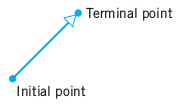
\includegraphics[scale=0.6]{imagens/vet001.png}
    %\footnotesize{Fonte:~}
  \end{center}
\end{figure}

\begin{itemize}[noitemsep]
\item A direção e o sentido da flecha indicam a \textbf{direção} e o
  \textbf{sentido} do vetor;
\item O comprimento da flecha indica a \textbf{magnitude} do vetor;
\item A cauda da flecha é o \textbf{ponto inicial} do vetor, sua origem;
\item A ponta da flecha é o \textbf{ponto final} do vetor, seu destino.
\end{itemize}

Existem inúmeras maneiras de representar um vetor em um texto, então a seguinte
convenção será utilizada aqui: os vetores serão representados por letras minúsculas
em negrito (\vet{a}, \vet{u}, \vet{v}, \ldots) e os escalares serão
representados por letras minúsculas em itálico (\esc{a}, \esc{k}, \esc{w}, \ldots).
Além disso, quando quisermos indicar que um determinado vetor \vet{v} tem origem
no ponto A e destino no ponto B, escrevemos: $\vet{v} = \overrightarrow{AB}$:

\begin{figure}[H]
  \begin{center}
    %\caption{}
    %\label{fig:}
    %\fbox{\includegraphics[scale=0.5]{imagens/.png}}
    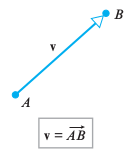
\includegraphics[scale=0.6]{imagens/vet002.png}
    %\footnotesize{Fonte:~}
  \end{center}
\end{figure}

Um vetor cujos pontos de origem e destino são os mesmos, por exemplo
$\vet{v} = \seta{AA}$, tem magnitude 0 e será chamado de \textbf{vetor zero}.
Tal vetor será representado por \vet{0}. ATENÇÃO: o vetor zero não tem direção
nem sentido definido, então fica convencionado que ele terá a direção e o sentido
mais conveniente à cada situação em particular. A mesma coisa ocorre para o número
de elmentos do vetor zero: ele terá tantos elementos $0$ quanto necessário para
a situação em particular.

%%%%%%%%%%%%%%%%%%%%%%%%%%%%%%%%%%%%%%%%%%%%%%%%%%%%%%%%%%%%%%%%%%%%%%%%%%%%%%%%%
\subsubsection{Equivalência (igualdade) de vetores}
\label{evd-geom-bi-tri-n-dimen-equiv}

Dados quaisquer vetores, eles serão \textbf{equivalentes} se, e somente se:
\begin{itemize}[noitemsep]
\item Tiverem a \emph{mesma magnitude}
\item Tiverem a \emph{mesma direção}
\item Tiverem o \emph{mesmo sentido}
\end{itemize}

Note que os vetores equivalentes são \textbf{iguais}, pois têm a mesma magnitude,
direção e sentido. Se dois vetores \vet{u} e \vet{v} são equivalentes, são
representados como: $\vet{u} = \vet{v}$.

Note também o seguinte: a LOCALIZAÇÃO dos vetores no espaço (bi, tri ou n-dimensional)
não tem influência
nenhuma na determinação da equivalência entre eles! Os vetores podem estar localizados
em locais completamente diferentes no espaço mas, se tiverem a mesma magnitude,
direção e sentido, são iguais. Por exemplo, a figura abaixo mostra vetores iguais
localizados em locais diferentes no espaço:

\begin{figure}[H]
  \begin{center}
    %\caption{}
    %\label{fig:}
    %\fbox{\includegraphics[scale=0.5]{imagens/.png}}
    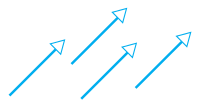
\includegraphics[scale=0.6]{imagens/vet003.png}
    %\footnotesize{Fonte:~}
  \end{center}
\end{figure}

%%%%%%%%%%%%%%%%%%%%%%%%%%%%%%%%%%%%%%%%%%%%%%%%%%%%%%%%%%%%%%%%%%%%%%%%%%%%%%%%%
\subsubsection{Soma de 2 vetores}
\label{evd-geom-bi-tri-n-dimen-soma-2}

Existem dois métodos para realizar a soma de 2 vetores de forma geométrica: o método
do \emph{paralelograma} e o método do \emph{triângulo}:

\begin{itemize}
\item \textbf{Método do Paralelograma}: se \vet{v} e \vet{w} são vetores no
  espaço bi- ou tri-dimensional e, se \emph{forem posicionados} de modo que o
  ponto de origem de ambos seja o mesmo, então os dois vetores formam os lados
  adjacentes de um paralelograma e a \emph{soma} $\vet{v} + \vet{w}$ será o vetor
  representado por uma flecha que sai do ponto de origem comum de \vet{v} e \vet{w}
  até o vértice oposto do paralelograma:
  \begin{figure}[H]
    \begin{center}
      %\caption{}
      %\label{fig:}
      %\fbox{\includegraphics[scale=0.5]{imagens/.png}}
      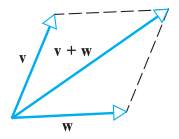
\includegraphics[scale=0.6]{imagens/vet004.png}
      %\footnotesize{Fonte:~}
    \end{center}
  \end{figure}
\item \textbf{Método do Triângulo}: se \vet{v} e \vet{w} são vetores no espaço bi-
  ou tri-dimensional e, se \emph{forem posicionados} de modo que o ponto inicial
  de \vet{w} coincida com o ponto final de \vet{v}, então a \emph{soma} $\vet{v}
  + \vet{w}$ será representada por uma flecha que sai do ponto inicial de \vet{v}
  até o ponto final de \vet{w}, formando um triângulo:
  \begin{figure}[H]
    \begin{center}
      %\caption{}
      %\label{fig:}
      %\fbox{\includegraphics[scale=0.5]{imagens/.png}}
      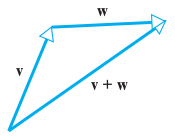
\includegraphics[scale=0.6]{imagens/vet005.png}
      %\footnotesize{Fonte:~}
    \end{center}
  \end{figure}
\end{itemize}

Note que a adição vetorial é \textbf{comutativa}, ou seja:

\begin{equation}
  \vet{v} + \vet{w} = \vet{w} + \vet{v}
\end{equation}

Prova geométrica de que a adição vetorial é comutativa:

\begin{figure}[H]
  \begin{center}
    %\caption{}
    %\label{fig:}
    %\fbox{\includegraphics[scale=0.5]{imagens/.png}}
    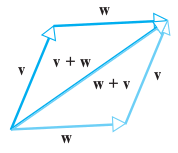
\includegraphics[scale=0.6]{imagens/vet006.png}
    %\footnotesize{Fonte:~}
  \end{center}
\end{figure}

%%%%%%%%%%%%%%%%%%%%%%%%%%%%%%%%%%%%%%%%%%%%%%%%%%%%%%%%%%%%%%%%%%%%%%%%%%%%%%%%%
\subsubsection{Soma de 3 ou mais vetores}
\label{evd-geom-bi-tri-n-dimen-soma-3+}

A soma vetorial, além de ser comutativa (como visto na seção anterior), é
\textbf{associativa}, de forma que a soma de três vetores \vet{u}, \vet{v} e \vet{w}
pode ser escrita como:

\begin{equation}
  \vet{u} + (\vet{v} + \vet{w}) = (\vet{u} + \vet{v}) + \vet{w}
\end{equation}

A soma de 3 ou mais vetores é feita, geometricamente, colocando-se a origem de um vetor na ``ponta''
do outro, e então desenhar o vetor resultante partindo da origem do primeiro vetor e
chegando na ponta do último. Por exemplo: a soma dos vetores \vet{u}, \vet{v}, \vet{w} e \vet{x}, dada por
$\vet{u} + \vet{v} + \vet{w} + \vet{x}$, é:

\begin{figure}[H]
  \begin{center}
    %\caption{}
    %\label{fig:}
    %\fbox{\includegraphics[scale=0.5]{imagens/.png}}
    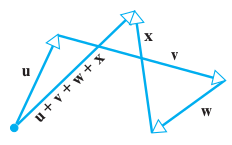
\includegraphics[scale=0.6]{imagens/vet010.png}
    %\footnotesize{Fonte:~}
  \end{center}
\end{figure}

Note que o método ilustrado acima pode ser entendido grosseiramente como
uma versão ``aumentada'' do método do triângulo para a soma de 2 vetores!

Se quisermos realizar a soma de 3 vetores em um espaço tridimensional com
um ponto de origem comum, a soma será a diagonal do paralelepípedo que tem
os vetores como lados adjacentes:

\begin{figure}[H]
  \begin{center}
    %\caption{}
    %\label{fig:}
    %\fbox{\includegraphics[scale=0.5]{imagens/.png}}
    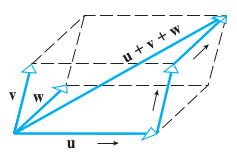
\includegraphics[scale=0.6]{imagens/vet011.png}
    %\footnotesize{Fonte:~}
  \end{center}
\end{figure}

Note também que o método ilustrado acima pode ser entendido grosseiramente
como uam versão ``aumentada'' do método do paralelograma para a soma de
2 vetores!

%%%%%%%%%%%%%%%%%%%%%%%%%%%%%%%%%%%%%%%%%%%%%%%%%%%%%%%%%%%%%%%%%%%%%%%%%%%%%%%%%
\subsubsection{Subtração de 2 vetores}
\label{evd-geom-bi-tri-n-dimen-subtracao-2}

A subtração de vetores utiliza um artifício aritmético que nos permite expressar
uma subtração em termos de uma soma. Por exemplo, sejam os escalares \esc{a} e
\esc{b}, podemos expressar a diminuição como:

\begin{equation}
  \esc{a} - \esc{b} = \esc{a} + (-\esc{b})
\end{equation}

Se \vet{w} e \vet{v} são vetores e queremos obter a subtração $\vet{w} - \vet{v}$,
basta calcularmos a soma de \vet{w} com o \emph{vetor oposto} de \vet{v}, o vetor
-\vet{v}:

\begin{equation}
  \vet{w} - \vet{v} = \vet{w} + (-\vet{v})
\end{equation}

E o que é o \emph{vetor oposto}? É um vetor que tem a mesma magnitude e direção,
mas sentido contrário. Matematicamente o vetor oposto é obtido pela multiplicação
do vetor original por $-1$. A figura abaixo mostra o vetor \vet{v} e o seu vetor oposto,
-\vet{v}:

\begin{figure}[H]
  \begin{center}
    %\caption{}
    %\label{fig:}
    %\fbox{\includegraphics[scale=0.5]{imagens/.png}}
    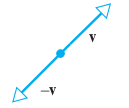
\includegraphics[scale=0.6]{imagens/vet007.png}
    %\footnotesize{Fonte:~}
  \end{center}
\end{figure}

Depois de obter o vetor oposto -\vet{v}, a subtração $\vet{w} - \vet{v}$ pode ser
resolvida expressando-a como a soma $\vet{w} + (-\vet{v})$ e utilizando o método
do paralelograma ou do triângulo (o resultado será o mesmo).

Se usarmos o método do paralelograma, o vetor $\vet{w} - \vet{v}$ será dado
pelo paralelograma formado com os vetores \vet{w} e -\vet{v}:

\begin{figure}[H]
  \begin{center}
    %\caption{}
    %\label{fig:}
    %\fbox{\includegraphics[scale=0.5]{imagens/.png}}
    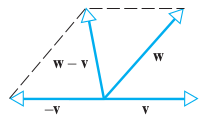
\includegraphics[scale=0.6]{imagens/vet008.png}
    %\footnotesize{Fonte:~}
  \end{center}
\end{figure}

Se usarmos o método do triângulo, o vetor $\vet{w} - \vet{v}$ será dado
pelo triângulo formado com os vetores \vet{w} e -\vet{v}:

\begin{figure}[H]
  \begin{center}
    %\caption{}
    %\label{fig:}
    %\fbox{\includegraphics[scale=0.5]{imagens/.png}}
    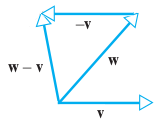
\includegraphics[scale=0.6]{imagens/vet009.png}
    %\footnotesize{Fonte:~}
  \end{center}
\end{figure}

Atenção: a subtração de vetores, em geral, \emph{não é comutativa}, ou seja:

\begin{equation}
  \vet{u} - \vet{v} \ne \vet{v} - \vet{u}
\end{equation}

Se a subtração for expressa como uma soma, a operação será comutativa:

\begin{equation}
  \vet{u} + (-\vet{v}) = (-\vet{v}) + \vet{u}
\end{equation}

%%%%%%%%%%%%%%%%%%%%%%%%%%%%%%%%%%%%%%%%%%%%%%%%%%%%%%%%%%%%%%%%%%%%%%%%%%%%%%%%%
\subsubsection{Subtração de 3 ou mais vetores}
\label{evd-geom-bi-tri-n-dimen-subtracao-3n}

A subtração de 3 ou mais vetores segue os mesmos princípios da subtração de 2
vetores, ou seja: expressamos os vetores através de seus opostos, e realizamos
a soma:

\begin{equation}
  \vet{u} - \vet{v} - \vet{x} = \vet{u} + (-\vet{v}) + (-\vet{x})
\end{equation}

%%%%%%%%%%%%%%%%%%%%%%%%%%%%%%%%%%%%%%%%%%%%%%%%%%%%%%%%%%%%%%%%%%%%%%%%%%%%%%%%%
\subsubsection{Multiplicação de um vetor por um valor escalar}
\label{evd-geom-bi-tri-n-dimen-multiplicacao-escalar}

Sempre que multiplicamos um vetor qualquer, \vet{u}, por um valor escalar
real qualquer, \esc{k}, estamos realizando a operação $\esc{k}\vet{u}$ e
o resultado desse \textbf{produto escalar} pode ser:

\begin{itemize}
\item Se $\esc{k} = 0$ ou se $\vet{u} = 0$: um vetor nulo (\vet{0});
\item Se $\esc{k} > 0$: um vetor com a mesma direção e sentido do vetor original, mas
  com a magnitude alterada por um fator \esc{k}, ou seja, a magnitude do vetor
  resultado será dada por $|\esc{k}| \times \vet{u}$;
\item Se $\esc{k} < 0$: um vetor com a mesma direção, mas com sentido \emph{oposto}
  ao do vetor original, e com a magnitude alterada por um fator \esc{k}, ou seja, a
  magnitude do vetor resultado será dada por $|\esc{k}| \times \vet{u}$.
\end{itemize}

A figura abaixo ilustra o produto escalar de um vetor \vet{v} com os escalares
$1/2$, $(-1)$, $2$, $(-3)$. Note que a magnitude do vetor é alterada por um fator
correspondente ao módulo do escalar ($|\esc{k}|$), a direção não é alterada,
e o sentido será o mesmo ou o oposto dependendo se o escalar é maior ou menor
do que zero:

\begin{figure}[H]
  \begin{center}
    %\caption{}
    %\label{fig:}
    %\fbox{\includegraphics[scale=0.5]{imagens/.png}}
    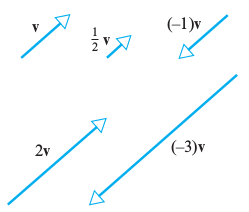
\includegraphics[scale=0.6]{imagens/vet012.png}
    %\footnotesize{Fonte:~}
  \end{center}
\end{figure}

Note que o produto escalar pode ser utilizado sempre que queremos alterar
a magnitude e/ou o sentido de um vetor.

%%%%%%%%%%%%%%%%%%%%%%%%%%%%%%%%%%%%%%%%%%%%%%%%%%%%%%%%%%%%%%%%%%%%%%%%%%%%%%%%%
\subsubsection{Vetores colineares e paralelos}
\label{evd-geom-bi-tri-n-dimen-paralelos}

Existe uma propriedade interessante do uso do conceito de produto escalar (a
multiplicação de um vetor por um valor escalar) que é a seguinte: se um vetor
\vet{w} for o produto escalar obtido a partir de um vetor \vet{v}, de forma que 
$\vet{w} = \esc{k}\vet{v}$, então eles são \emph{colineares}:

\begin{figure}[H]
  \begin{center}
    %\caption{}
    %\label{fig:}
    %\fbox{\includegraphics[scale=0.5]{imagens/.png}}
    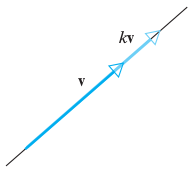
\includegraphics[scale=0.6]{imagens/vet013.png}
    %\footnotesize{Fonte:~}
  \end{center}
\end{figure}

Agora note o seguinte: por definição, a LOCALIZAÇÃO de um vetor no espaço
não é importante! Assim o produto escalar, além de ser considerado colinear,
também pode ser considerado como \emph{paralelo}:

\begin{figure}[H]
  \begin{center}
    %\caption{}
    %\label{fig:}
    %\fbox{\includegraphics[scale=0.5]{imagens/.png}}
    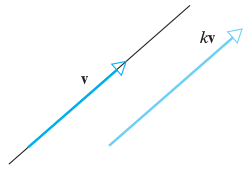
\includegraphics[scale=0.6]{imagens/vet014.png}
    %\footnotesize{Fonte:~}
  \end{center}
\end{figure}

Isso causa uma certa confusão pois na matemática ``normal'' colinear não é a
mesma coisa que paralelo. Mas, quando se trata de vetores, somos obrigados a
considerar que colinear significa a mesma coisa que paralelo! Em resumo: se
um vetor é o produto escalar de outro, eles são paralelos (ou colineares)!



%%%%%%%%%%%%%%%%%%%%%%%%%%%%%%%%%%%%%%%%%%%%%%%%%%%%%%%%%%%%%%%%%%%%%%%%%%%%%%%%%
%%%%%%%%%%%%%%%%%%%%%%%%%%%%%%%%%%%%%%%%%%%%%%%%%%%%%%%%%%%%%%%%%%%%%%%%%%%%%%%%%
%%%%%%%%%%%%%%%%%%%%%%%%%%%%%%%%%%%%%%%%%%%%%%%%%%%%%%%%%%%%%%%%%%%%%%%%%%%%%%%%%
%%%%%%%%%%%%%%%%%%%%%%%%%%%%%%%%%%%%%%%%%%%%%%%%%%%%%%%%%%%%%%%%%%%%%%%%%%%%%%%%%
%%%%%%%%%%%%%%%%%%%%%%%%%%%%%% TERMINA O DOCUMENTO %%%%%%%%%%%%%%%%%%%%%%%%%%%%%%
%%%%%%%%%%%%%%%%%%%%%%%%%%%%%%%%%%%%%%%%%%%%%%%%%%%%%%%%%%%%%%%%%%%%%%%%%%%%%%%%%
%%%%%%%%%%%%%%%%%%%%%%%%%%%%%%%%%%%%%%%%%%%%%%%%%%%%%%%%%%%%%%%%%%%%%%%%%%%%%%%%%
%%%%%%%%%%%%%%%%%%%%%%%%%%%%%%%%%%%%%%%%%%%%%%%%%%%%%%%%%%%%%%%%%%%%%%%%%%%%%%%%%
%%%%%%%%%%%%%%%%%%%%%%%%%%%%%%%%%%%%%%%%%%%%%%%%%%%%%%%%%%%%%%%%%%%%%%%%%%%%%%%%%
\end{document}









